\newpage
\section{Fourierreihe periodischer Signale}
\subsection{Reelle Fourierreihe (FR)}
		
{\small $a_k, b_k$: FR-Koeffizienten.\\
	$k=0$: Gleichanteil, Mittelwert.\\
	$k=1$: Grundschwingung, 1.Harmonische.\\
	$k=n$: $n$.Harmonische, ($n-1$).Oberschwingung.}
	\begin{itemize}
		\item Synthese, trigonometrische Form:
		      \[
			      x(t) = \frac{a_0}{2} + \sum_{k=1}^\infty [a_k\cdot \cos(k\omega_1 t)+ b_k\cdot \sin(k\omega_1 t)]
		      \]
		\item Synthese, harmonische Form:\\
				{\small $A_k$: Gewichte, Amplituden}
		      \begin{align*}
			      x(t) & = A_0+\sum_{k=1}^\infty A_k\cdot \sin (k\omega_1 t + \alpha_k)              \\
			           & = A_0+\sum_{k=1}^\infty A_k\cdot \cos (k\omega_1 t -( \underbrace{-\alpha_k+\frac{\pi}{2} }_{\beta_k}))\\
			           & = \boxed{A_0+\sum_{k=1}^\infty A_k\cdot \cos (k\omega_1 t + \varphi_k)}\\
  			           & = A_0+\sum_{k=1}^\infty A_k \cdot \sin (k\omega_1 t + \varphi_k - \frac{\pi}{2})
		      \end{align*}

		\item Analyse, trigonometrische Form:
		\begin{gather*}
		      	\text{Gleichanteil: }\frac{a_0}{2}= A_0 = \frac{1}{T}\int_{t_0}^{T+t_0} x(t)dt\\
			      a_k = \frac{2}{T}\int_{t_0}^{T+t_0} x(t)\cdot \cos(k\omega_1 t)\,dt \\
			      b_k = \frac{2}{T}\int_{t_0}^{T+t_0} x(t)\cdot \sin(k\omega_1 t)\,dt
		\end{gather*}
		\item Umwandlung Harmonisch $\Leftrightarrow$ Trigonometrisch:
		\begin{gather*}
			A_0 = \frac{a_0}{2} = \underline{c}_0 \quad
			A_k = \sqrt{a_k^2+b_k^2}\\
			a_k = A_k \sin(\alpha_k) = A_k \cos(\beta_k) = A_k \cos(\varphi_k)\\
			%\quad \tan(\beta_k)=\frac{b_k}{a_k} \\
			b_k = A_k \cos(\alpha_k) = A_k \sin(\beta_k) = - A_k \sin(\varphi_k)\\
			\tan(\alpha_k)=\frac{a_k}{b_k} \quad \tan(\beta_k)=\frac{b_k}{a_k} \quad \tan(\varphi_k)=\frac{-b_k}{a_k}
		\end{gather*}
		Vereinfachung durch Nutzung der Symmetrieeigenschaften $\rightarrow$ siehe Kap. XX.
	\end{itemize}

\subsection{Komplexe Fourierreihe}
	\begin{itemize}
		\item Synthese: $\omega \rightarrow t$
		{\small\quad $\underline{c}_k$: Gewichte}
		\[
		x(t)= \sum_{k=-\infty}^{\infty} \underline{c}_k\cdot e^{jk \omega_1  t} \text{ mit } \underline{c}_k = |\underline{c}_k|\cdot e^{j\varphi_k}
		\]
		\item Analyse: $t \rightarrow \omega$
		\begin{align*}
			\underline{c}_k & = \frac{1}{T}\int_{t_0}^{t_0+T} x(t)\cdot e^{-jk\omega_1  t}dt
			& = \boxed{\frac{1}{T} \cdot \underline{X}(k\omega_1) }
		\end{align*}
	\item Umwandlung Komplex $\Leftrightarrow$ Reell.
	\begin{gather*}
		\frac{a_0}{2} = A_0 = \underline{c}_0 \quad A_k = 2|\underline{c}_k| \quad \beta_k = -\varphi_k\\
			a_k = 2\ \mathfrak{Re}\left\{ \underline{c}_k \right\}= \left[ \underline{c}_k+\underline{c}_{-k} \right]\\
			b_k = -2\ \mathfrak{Im}\left\{ \underline{c}_k \right\}= j\left[ \underline{c}_k-\underline{c}_{-k} \right]\\
			\underline{c}_k = \frac{1}{2}\left( a_k-jb_k \right) = \frac{A_k}{2} e^{-j\beta_k} = \frac{A_k}{2} e^{j\varphi_k}\\
			\underline{c}_{-k} = \frac{1}{2}\left( a_k+jb_k \right) = \frac{A_k}{2} e^{j\beta_k} = \frac{A_k}{2} e^{-j\varphi_k}
	\end{gather*}
	\end{itemize}




\subsection{Symmetrieeigenschaften}
\begin{itemize}
	\item \textbf{Gerade} Funktionen
	      - symmetrisch zur y-Achse\\
	     {\small Alle $sin$-Anteile verschwinden.}
	     \begin{align*}
	     	b_k &=0 \qquad
	     	A_0 = \frac{2}{T}\int^{\frac{T}{2}}_{0} y(t)\,dt\\
	     	a_{k} &= \frac{4}{T}\int^{\frac{T}{2}}_{0}y(t)\cdot \cos(k\omega_1t)\,dt
	     \end{align*}
	\item \textbf{Ungerade} Funktionen
	      - symmetrisch zum Ursprung\\
	  		{\small Gleichanteil und alle $cos$-Anteile verschwinden.}
	      \begin{align*}
	      	a_k &=0 \qquad
	      	A_0 = 0\\
	      	b_{k} &= \frac{4}{T}\int^{\frac{T}{2}}_{0}y(t)\cdot \sin(k\omega_1t) dt
	      \end{align*}
\end{itemize}
\subsubsection{Halbwellensymmetrie}
{\small FR mit HWS enthält nur ungerade Terme: $\rightarrow k=1,3,5,\dots,\infty$}
\begin{itemize}
	
	\item Allgemein: $y(t) = -y(t \pm T/2)$
	\begin{align*}
		A_0 &= 0,\quad
		a_{2k} = 0,\quad
		b_{2k} = 0\\
		a_{2k-1} &= \frac{4}{T}\int^{\frac{T}{2}}_{0}y(t)\cdot \cos((2k-1)\,\omega_1t)\,dt\\
		b_{2k-1} &= \frac{4}{T}\int^{\frac{T}{2}}_{0}y(t)\cdot \sin((2k-1)\,\omega_1t)\,dt
	\end{align*}
	
	\item gerade Halbwellensymmetrie:
		\begin{align*}
		A_0 &= 0,\quad
		b_k = 0,\quad
		a_{2k} = 0\\
		a_{2k-1} &= \frac{8}{T}\int^{\frac{T}{4}}_{0}y(t)\cdot \cos((2k-1)\,\omega_1t)\,dt
	\end{align*}
	
		\item ungerade Halbwellensymmetrie:
	\begin{align*}
	A_0 &= 0,\quad
	a_k = 0,\quad
	b_{2k} = 0\\
	b_{2k-1} &= \frac{8}{T}\int^{\frac{T}{4}}_{0}y(t)\cdot \sin((2k-1)\,\omega_1t)\,dt
	\end{align*}
\end{itemize}

\subsection{Verschiebungssatz}
\textbf{Zeit}verschiebung $\Leftrightarrow$ \textbf{Phasen}drehung im Freq.-bereich um den Winkel: $-k\omega_1 t_v$
\begin{align*}
	f_v(t) = f(t-t_v) & = \sum_{k=-\infty}^{\infty} \underline{c}_k\cdot e^{j\omega_1 k (t-t_v)}                                                       \\
	                  & = \sum_{k=-\infty}^{\infty} \underbrace{\underline{c}_k\cdot e^{-j\omega_1 k t_v}}_{\underline{c}_{k_v}} \cdot e^{\omega_1 k t}
\end{align*}

$t_v$ < 0: Phasenwinkel des Spektrums werden\\ mit
zunehmender Frequenz größer.

\subsection{FR und LTI-Systeme}
{\small LTI-Systeme verändern Betrag und Phase aller harmonischen Komponenten eines Eingangssignals = lineare Verzerrung.\\
Sie fügen \underline{keine} neuen Frequenzen hinzu.}
\[
	y(t) = \sum_{k=-\infty}^{\infty} \underbrace{\underline{H}(k\omega_1)\cdot\underline{c}_{xk}}_{\underline{c}_{yk}} \cdot e^{j\omega_1 k t}
\]
\subsection{FR-Tabelle - Bischoff}
\begin{itemize}[leftmargin=*]
	\item normierte Pulsbreite $p=\dfrac{|\Delta t|}{T} = \frac{\texttt{Länge Zeit}}{\texttt{Periodendauer}}$
	\item $\overline{|f(t)|}$: Mittelwert Wechselanteil/ Gleichrichtwert.
	\item $f_{\texttt{eff}}$: \underline{Gesamt}-Effektivwert des Signals.
	\item FR-Reihen sind auf Amplitude $\hat{f}$ normiert!\\ $\rightarrow$ mit $\hat{f}$ multiplizieren!
\end{itemize}
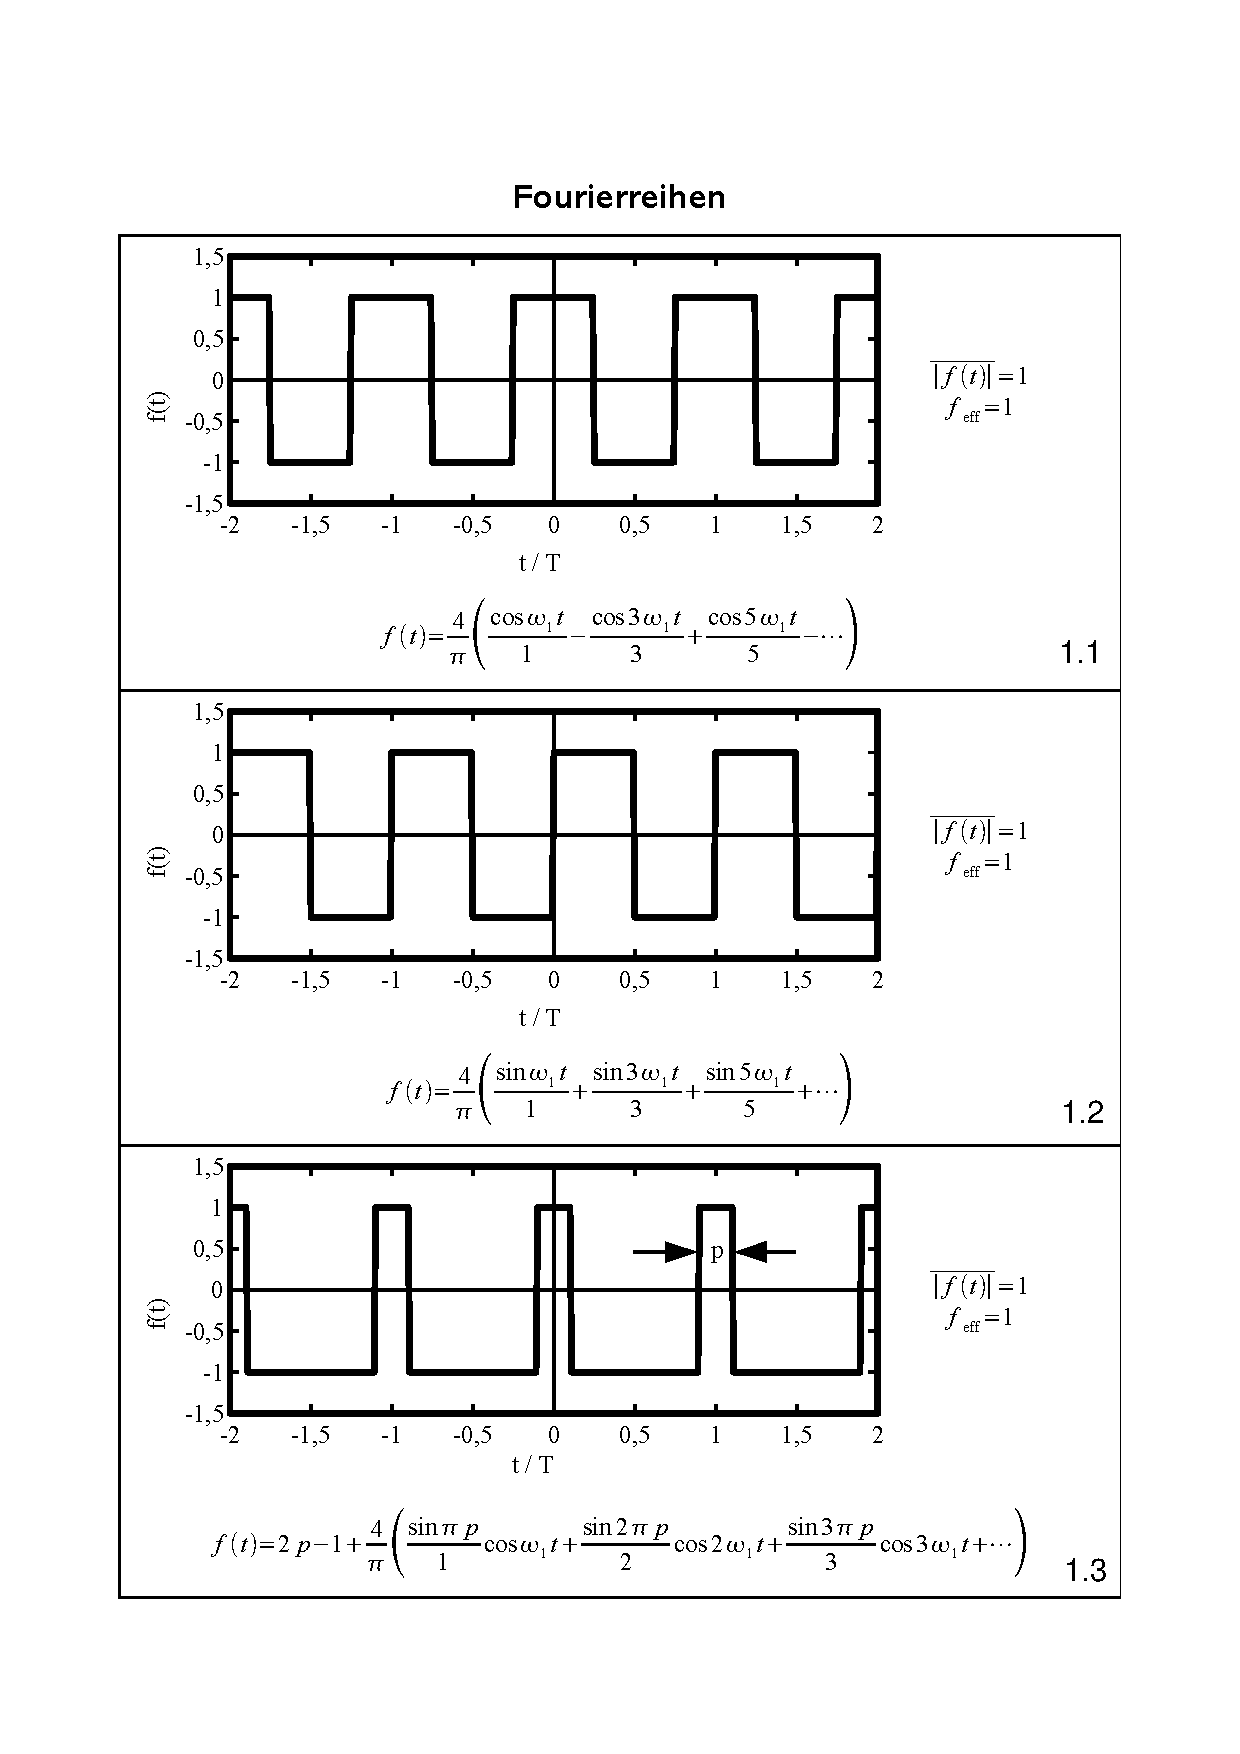
\includegraphics[page=1,width=\columnwidth]{./Bilder/Fourierreihen_Bischoff_V2}
\includegraphics[page=2,width=\columnwidth]{./Bilder/Fourierreihen_Bischoff_V2}
\includegraphics[page=3,width=\columnwidth]{./Bilder/Fourierreihen_Bischoff_V2}
\includegraphics[page=4,width=\columnwidth]{./Bilder/Fourierreihen_Bischoff_V2}\\
\includegraphics[page=5,width=\columnwidth]{./Bilder/Fourierreihen_Bischoff_V2}\\
\includegraphics[page=6,width=\columnwidth]{./Bilder/Fourierreihen_Bischoff_V2}\\
\includegraphics[page=7,width=\columnwidth]{./Bilder/Fourierreihen_Bischoff_V2}\\
\includegraphics[page=8,width=\columnwidth]{./Bilder/Fourierreihen_Bischoff_V2}\\
\includegraphics[page=9,width=\columnwidth]{./Bilder/Fourierreihen_Bischoff_V2}\\


\newpage
\subsection{Kenngrößen periodischer Signale}
\subsubsection{Effektivwert, Klirrfaktor, Mischgrößen}
\begin{itemize}
	\item \textbf{Effektivwert}:
	{\small Wert einer Gleichgröße, die im Mittel die gleiche elek. Leistung an einem $R$ umsetzt.}
\begin{gather*}
		      U_{\mathit{eff}} = U = \sqrt{\frac{1}{T} \int_\tau^{\tau+T} u(t)^2 dt} = \sqrt{U_{\sim}^2+U_{0}^2}\\
		      \text{Sinusf\"ormige Signale: }U_k = \frac{\hat{u}_k}{\sqrt{2}}
\end{gather*}
$U_\sim:$ Wechselanteil \quad $U_0$: Gleichanteil, Mittelwert
 	\item Effektivwert mit \textbf{Fourier-Reihe}:\\
		  $$ U_{\mathit{eff}} = \sqrt{\sum_{k=-\infty}^{\infty} c_k^2} = \sqrt{\sum_{k=0}^{\infty}U_{k,\mathit{eff}}^2} = \sqrt{U_0^2 + \frac{1}{2} \sum_{k=1}^{\infty} \hat{u}_k^2}$$
	\item \textbf{Klirrfaktor}, Oberschwingungsgehalt:\\
	      {\small Maß für Abweichung eines Signals $x(t)$ von der $\sin$-Form. Angabe von $k$ in \%. Kein Gleichanteil $U_0=0$.}
	      \begin{align*}
		      k & = \frac{\texttt{\small Effektivwert  Oberschwingungen}}{\texttt{\small Effektivwert Wechselanteil}}\leq 1\\
		        & = \frac{\sqrt{\sum_{{\color{red}{k=2}}}^{\infty} U_{k}^{2}}}{\sqrt{\sum_{{\color{red}{k=1}}}^{\infty} U_{k}^{2}}} = \frac{\sqrt{U_\sim^2 - U_1^2}}{U_\sim} \\
		        & = \sqrt{\frac{0,5 \cdot \sum_{k=2}^{\infty}\hat{u}_k^2}{0,5 \cdot \sum_{k=1}^{\infty}\hat{u}_k^2}} \text{\small \quad mit FR-Amplituden } \hat{u}_k\\
		        & = \sqrt{1-\frac{U_1^2}{U_\sim^2}} = \sqrt{1-g^2} \quad \text{mit } g = \frac{U_1}{U_\sim}\\
		      k_m &= \frac{U_m}{U_\sim} \qquad k_1 = g = \sqrt{1-k^2}
	      \end{align*}
{\small Für Wechselgrößen lässt sich $k$ einfach mit \textbf{Grundschwingungsgehalt} $g$ ermitteln (\textit{gilt immer}).}
	\item \textbf{Mischgrößen:}\\
	      - Schwingungsgehalt:
	      \[
		      s = \frac{U_\sim}{U} = \frac{\texttt{Effektivwert des Wechselanteils}}{\texttt{Effektivwert der Mischgröße}}
	      \]
	      - Welligkeit:
	      \[
		      w = \frac{U_\sim}{\bar{U}} = \frac{\texttt{Effektivwert des Wechselanteils}}{\texttt{Gleichanteil}}
	      \]
	      - Riffelfaktor:
	      \[
		      R = \frac{\hat{U}_\sim}{\bar{U}} = \frac{\texttt{Scheitelwert des Wechselanteils}}{\texttt{Gleichanteil}}
	      \]
\end{itemize}
\subsubsection{Leistungen}
\begin{itemize}  
	\item \textbf{Wirkleistung}:
\begin{align*}
			      P & = \bar{p}(t) = \frac{1}{T} \int_0^T u(t)\cdot i(t) dt
     		       = \sum_{k=-\infty}^{\infty}\underline{u}_k \underline{i}_k^* \leftrightarrow i_k^* = i_{-k}\\
     		       &= 
  			      P_0 + \sum_{k=1}^{\infty} U_{k_{\mathit{eff}}}\cdot
     		       I_{k_{\mathit{eff}}}\cdot\cos(\varphi_{u,k}-\varphi_{i,k})\\
     		       &= U_0 \cdot I_0 + \sum_{k=1}^{\infty} \frac{\hat{u}_k\cdot \hat{i}_k}{2} \cdot \cos(\varphi_{u,k}-\varphi_{i,k})\\
     		       & = \frac{U^2}{R}= I^2 \cdot R \text{\qquad rein am ohmschen Widerstand!}
\end{align*} 
		\item \textbf{Blindleistung}\\
		{\small Nicht-sinusf\"ormige Gr\"o\ss en: $Q$ ist vorzeichenlos! $[Q]=\texttt{var}$}
		\begin{gather*}
			|Q| = \sqrt{Q^2_v + D^2} = \sqrt{S^2-P^2}
		\end{gather*}
		
	      \begin{mdframed}[style=exercise,frametitle=Verschiebungs-/Feldblindleistung $Q_v$]
	      	\[
	      	Q_v = \sum_{k=1}^{\infty} U_k \cdot I_k \cdot \sin(\varphi_{u,k}-\varphi_{i,k})
	      	\]
{\small Gleiche Frequenz, aber Phasenverschiebung zwischen $U$ und $I$.}
	      \end{mdframed}
	      
	      
	      \begin{mdframed}[style=exercise,frametitle=Verzerrungsblindleistung $D$]
	      		      {\small auch Oberwellen-, Deformationsblindleistung.}
		      \[
			      D^2 = U_1^2\cdot(I^2-I_1^2) = S^2(1-g^2)
		      \]
\small{aus Mischtermen als Produkte von $U$ und $I$ unterschiedlicher Frequenzen.}
	      \end{mdframed}
  		\item \textbf{Scheinleistung}\\
{\small Gilt auch f\"ur Mischgr\"o\ss en, da Effektivwerte Gleichanteile enthalten k\"onnen. Achtung: $U, I$: \textbf{Gesamt}signal!}
\begin{align*}
	      S &= U_{\mathit{eff}}\cdot I_{\mathit{eff}} = U\cdot I = \sqrt{P^2+Q^2} = \sqrt{P^2+Q_v^2+D^2}\\
	      &=  \sqrt{\sum_{k=0}^{+\infty} U_k^2} \cdot \sqrt{\sum_{k=0}^{+\infty} I_k^2} = \sqrt{\left( \sum_{k=0}^{+\infty} U_k^2 \right) \cdot \left( \sum_{k=0}^{+\infty} I_k^2 \right)}\\
	      &\neq \sqrt{\sum_{k=0}^{+\infty} U_k^2 \cdot I_k^2}
\end{align*}
	      	Nicht-linearer Verbraucher an einer sinusförmigen Spannung $U_1$:
	      	\vspace{-1.5em}
	      	\begin{multline*}
	      		S^{2}=(U I)^{2}=U_{1}^{2} \cdot \sum_{k=0}^{\infty} I_{k}^{2}=\\U_{1}^{2} I_{0}^{2}+U_{1}^{2} \sum_{k=2}^{\infty} I_{k}^{2}+U_{1}^{2} I_{1}^{2} \sin ^{2} \varphi_{1}+U_{1}^{2} I_{1}^{2} \cos ^{2} \varphi_{1}
	      	\end{multline*}
	      Räumliche Darstellung der Leistungen:
	      \begin{center}
	      	\vspace{-0.5em}
	      	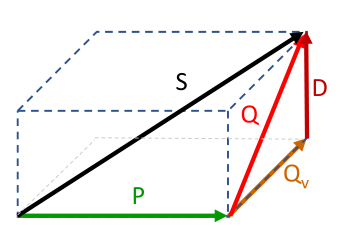
\includegraphics[width=0.35\columnwidth]{Schein-Blindleistung_raeumlich.png}
	      	\vspace{-0.6em}
	      \end{center}
	      \item \textbf{Leistungsfaktor}:
\begin{align*}
	\text{\small Allgemein: }
	      \lambda &= \frac{|P|}{S} = \sqrt{1-\frac{Q^2}{S^2}} \quad 0<\lambda<1\\
	     \text{\small Sinusf\"ormig: }\lambda &= \frac{P}{S}=\cos(\varphi)=\cos(\varphi_u-\varphi_i)
\end{align*}
\end{itemize}
\clearpage
\section{Fourier-Transformation (FT)}
\subsection{Hin- und Rücktransformation}
{\small Übertragung (nicht-)periodischer Signale in Spektrum/BB.}\\
\begin{mdframed}[style=exercise]
	\small { \textbf{Bedingung}: $x(t)$ absolut integrierbar! $\int_{t=-\infty}^{+\infty}|x(t)|dt<\infty$ }
	\[
		x(t) \quad \laplace  \quad \underline{X}(\omega)
	\]
	Hintransformation - Analysegleichung:
	\[
		\underline{X}(\omega)=\mathcal{F}\left\{ x(t) \right\} = \int_{-\infty}^{\infty} x(t) \cdot e^{-j\omega t} dt
	\]
	Rücktransformation - Synthesegleichung:
	\[
		x(t) = \mathcal{F}^{-1}\left\{ \underline{X}(\omega) \right\} = \frac{1}{2\pi}\int_{-\infty}^{\infty} \underline{X}(\omega) \cdot e^{j\omega t} d\omega
	\]
	Komplexwertige Fouriertransformierte:
	\[
	\underline{X}(\omega) = |\underline{X}(\omega)|\cdot e^{j\omega\varphi}
	\]
	\footnotesize
	Einheit: Amplitudendichte $\left[ x(t) \right]\cdot s$
	\normalsize
	
\end{mdframed}

\subsection{FT periodischer Signale}
\begin{itemize}

	\item Übergang FR $\rightarrow$ FT:
\begin{align*}
	U_a(\omega) &= 2\pi \cdot \sum_{k=-\infty}^{+\infty} \underline{c}_k \cdot \delta(\omega-k\omega_a)\\
	& = 2\pi \cdot \sum_{k=-\infty}^{+\infty} \frac{\underline{U}(\omega)}{t_a} \cdot \delta(\omega-k\omega_a)\\
	&= \frac{2\pi}{t_a} \cdot \sum_{k=-\infty}^{+\infty} \underline{U}(\omega) \cdot \delta(\omega-k\omega_a) \\
	& =  \omega_a \cdot \sum_{k=-\infty}^{+\infty} \underline{U}(\omega-k\omega_a)
\end{align*}
	\item Übergang FT $\rightarrow$ FR, Komplexe Fourierkoeffizienten, periodische Fortsetzung:
	\[ \boxed{
		\quad \underline{c}_k =
		\frac{1}{T} \cdot \underline{X}(k\omega_1) } =
		\frac{1}{T}\int_0^T x(t) \cdot e^{-j\omega_1 t} dt
	\]
	\small{$T=t_p$: Periodizität, Periodendauer.}\\
	\small{ $\underline{c}_k$: FR-Koeff. d. periodischen Fortsetzung \\des endlichen Signals $x(t)$ mit Länge $T$.}\\
	
	\item FR-Koeffizienten $\underline{c}_k $ sind
	\textbf{Abtastwerte} von $\underline{X}(\omega)$ bei den Frequenzen im Linienabstand:
	\[\omega=k\omega_1=k\frac{2\pi}{T}=k\frac{2\pi}{t_p}\]
\end{itemize}

\subsection{Zeit-Bandbreite-Gesetz}

%\subsubsection{Eigenschaften der FT}
%	\begin{itemize}
%		\item \textbf{Linearität}
%		      \[
%			      A x_{1}(t)+ B x_{2}(t)\ \laplace\  A \cdot  \underline{X}_{1}(\omega)+B \cdot \underline{X}_{2}(\omega)
%		      \]
%		      % {\footnotesize Eine lineare Überlagerung von gewichteten Zeitsignalen führt zur linearen
%		      % Überlagerung der Spektren mit denselben Vorfaktoren.}
%		\item \textbf{Dualität}
%		      \[
%			      \underline{X}(t)\ \laplace\  2\pi\cdot x(-\omega)
%		      \]
%		      % {\footnotesize Zeit- und Frequenzbereich können vertauscht werden (bis auf den Faktor $2\pi$
%		      % und einer Vorzeichenumkehr).}
%		\item \textbf{Zeitskalierung}
%		      \[
%			      x(a \cdot t)\ \laplace\ \frac{1}{|a|} \underline{X}\left(\frac{\omega}{a}\right) \quad a \in \mathbb{R} \backslash\{0\}
%		      \]
%		      % {\footnotesize Eine Stauchung der Zeitachse führt zur Dehnung der Frequenzachse.
%		      % Frequenzachse (und Skalierung der Amplitude).}
%		\item \textbf{Frequenzskalierung}
%		      \[
%			      \frac{1}{|b|} x\left(\frac{t}{b}\right)\ \laplace\ \underline{X}(b\cdot\omega) \quad b \in \mathbb{R} \backslash\{0\}
%		      \]
%		      % {\footnotesize Eine Stauchung der Frequenzachse führt zur Dehnung der Zeitachse.
%		      % Zeitachse (und Skalierung der Amplitude).}
%		\item \textbf{Zeitverschiebung}
%		      \[
%			      x\left(t-t_{0}\right)\ \laplace\ \underline{X}(\omega) \cdot e^{-j \omega t_{0}}
%		      \]
%		      % {\footnotesize Eine Verschiebung im Zeitbereich ändert nicht den Betrag des Spektrums,
%		      % aber die Phase um einen sich mit der Frequenz $\omega$ linear ändernden Phasenterm.}
%		\item \textbf{Frequenzverschiebung - Modulation}
%		      \[
%			      x(t) \cdot e^{j \omega_{0} t}\ \laplace\ \underline{X}\left(\omega-\omega_{0}\right)
%		      \]
%		      % {\footnotesize Eine Verschiebung im Frequenzbereich führt zu einem Modulationsterm im
%		      % Zeitbereich oder andersherum, um eine Frequenzverschiebung zu erreichen,
%		      % muss im Zeitbereich mit $e^{(j\omega_0t)}$ multipliziert (moduliert) werden.}
%		\item \textbf{Faltung}
%		      \[
%			      x_{1}(t) * x_{2}(t)\ \laplace\ \underline{X}_{1}(\omega) \cdot \underline{X}_{2}(\omega)
%		      \]
%		      % {\footnotesize Faltung im Zeitbereich entspricht Multiplikation im Frequenzbereich}
%		\item \textbf{Multiplikation - Fenstertheorem}
%		      \[
%			      x_{1}(t) \cdot x_{2}(t)\ \laplace\ \frac{1}{2 \pi} \underline{X}_{1}(\omega) * \underline{X}_{2}(\omega)
%		      \]
%		      % {\footnotesize Multiplikation im Zeitbereich entspricht Faltung im Frequenzbereich (und
%		      % Normierung mit $2\pi$).}
%		\item \textbf{Differentiation\\}
%		      {\small im Zeitbereich:}
%		      \[
%			      \frac{d}{dt} x(t) \ \laplace\ j\omega\underline{X}(\omega)
%		      \]
%		      {\small im Frequenzbereich:}
%		      \[
%			      t \cdot x(t)\ \laplace\ j \frac{d}{d \omega} \underline{X}(\omega)
%		      \]
%		      % {\footnotesize Differenzieren im Zeitbereich dreht die Phase des Spektrums um $\frac{\pi}{2}$ und
%		      % verstärkt die Amplitude des Spektrums zu hohen Frequenzen hin mit linear
%		      % anwachsendem $\omega$.}
%		\item \textbf{Integration}
%		      \[
%			      \int_{-\infty}^{t} x(\tau) d \tau\ \laplace\ \frac{1}{j \omega} \underline{X}(\omega)+\pi \cdot \underline{X}(0) \cdot \delta(\omega)
%		      \]
%		      % {\footnotesize Integrieren dreht die Phase um $-\frac{\pi}{2}$, dämpft die Amplitude des
%		      % Spektrums mit $\frac{1}{\omega}$ und erzeugt einen (dem Gleichanteil von
%		      % $x(t)$ entsprechenden) Dirac bei $\omega = 0$.}
%		\item \textbf{Energieberechnung - Parseval}
%		      \[
%			      \int_{-\infty}^{+\infty}|x(t)|^{2} d t=\frac{1}{2 \pi} \int_{-\infty}^{+\infty}|\underline{X}(\omega)|^{2} d \omega
%		      \]
%		      % {\footnotesize Die Signalenergie lässt sich aus der Zeit- und Frequenzbereichsdarstellung berechnen.}
%	\end{itemize}
\clearpage
\subsection{Eigenschaften der FT}
\begin{tabularx}{1.03\columnwidth}{|X|c|c|}
	\hline & $x(t)$ & $\mathbf{\underline{X}(\omega)}$ \\
	\hline Linearität & $A x_{1}(t)+B x_{2}(t)$ & $A \underline{X}_{1}(\omega)+B \underline{X}_{2}(\omega)$ \\
	\hline  Verschiebung & $x(t-t_0)$ & $e^{-j \omega t_0} \underline{X}(\omega)$ \\
	\hline Modulation & $e^{j \omega_{0} t} x(t)$ & $\underline{X}\left(\omega-\omega_{0}\right)$ \\
	\hline 
		\small Differentiation im Frequenzbereich
	 & $t \cdot x(t)$ & $j \dfrac{d \underline{X}(\omega)}{d \omega}$ \\
	\hline 
		\small Differentiation
		im Zeitbereich & $\frac{d x(t)}{d t}$ & $j \omega \underline{X}(\omega)$ \\
	\hline Integration & $\int_{-\infty}^{t} x(\tau) d \tau$ & $\frac{1}{j \omega} \underline{X}(\omega)+\pi \underline{X}(0) \delta(\omega)$ \\
	\hline Zeitskalierung & $x(a t)$ & $\frac{1}{|a|} \underline{X}\left(\frac{\omega}{a}\right), \quad a \in \mathbb{R} \backslash\{0\}$ \\
	\hline \textbf{Faltung} & $x_{1}(t) * x_{2}(t)$ & $\underline{X}_{1}(\omega) \cdot \underline{X}_{2}(\omega)$ \\
	\hline Multiplikation & $x_{1}(t) \cdot x_{2}(t)$ & $\dfrac{1}{2 \pi} \underline{X}_{1}(\omega) * \underline{X}_{2}(\omega)$ \\
	\hline Dualität & \begin{tabular}{l}
		$x_{1}(t)$ \\
		$x_{2}(t)$
	\end{tabular} & \begin{tabular}{l}
		$x_{2}(\omega)$ \\
		$2 \pi x_{1}(-\omega)$
	\end{tabular} \\
	\hline Symmetrien & \begin{tabular}{c}
		$x(-t)$ \\
		$x^{*}(t)$ \\
		$x^{*}(-t)$
	\end{tabular} & \begin{tabular}{c}
		$\dfrac{X}{X^{*}}(-\omega)$ \\
		$\underline{X}^{*}(\omega)$
	\end{tabular} \\
	\hline Parsevalsches Theorem & $\int_{-\infty}^{\infty}|x(t)|^{2} d t$ & $\frac{1}{2 \pi} \int_{-\infty}^{\infty} \left|\underline{X}(\omega) \right| $\\
	\hline	
\end{tabularx}


\subsection{Faltungsregeln}
\normalsize
\begin{itemize}
	\item {$a*b=b*a$} {\small \qquad kommutativ}
	\item $a*[b*c]=[a*b]*c$
	\item $a\cdot(f*g)=(a\cdot f) * g = f * (a\cdot g)$
	\item $a*[b+c]=a*b+a*c$
	\item $x(t) * \delta(t-t_0) = x(t-t_0)$ {\small \qquad Ausblendeigenschaft}
\end{itemize}

\subsection{Transformationspaare der FT}
\begin{tabularx}{0.95\columnwidth}{|c|X|}
	\hline$x(t)$ & $\mathbf{\underline{X}(\omega)}$ \\
	\hline$\delta(t)$ & 1 \\
	\hline 1 & $2 \pi \cdot \delta(\omega)$ \\
	\hline$\dot{\delta}(t)$ & $j \omega$ \\
	\hline$\sum_{m=-\infty}^{\infty} \delta(t-m T)$ & $\omega_{1} \cdot \sum_{k=-\infty}^{\infty} \delta\left(\omega-k \omega_{1}\right) \quad$ mit $\omega_{1}=\frac{2 \pi}{T}$ \\
	\hline$\varepsilon(t)$ & $\pi \delta(\omega)+\frac{1}{j \omega}$ \\
	\hline $\operatorname{rect}\left(\frac{t}{2 a T}\right)$ & $2 aT \cdot \operatorname{si}(\omega aT)$ \\
	\hline $\operatorname{si}(a t)$ & $\frac{\pi}{|a|} \operatorname{rect}\left(\frac{\omega}{2 a}\right)$ \\
	\hline$\frac{|a|}{\pi} \operatorname{si}(a t)$ & $\operatorname{rect}\left(\frac{\omega}{2 a}\right)$ \\
	\hline$\dfrac{1}{t}$ & $-j \pi \operatorname{sign}(\omega)$ \\
	\hline $\operatorname{sign}(t)$ & $\frac{2}{j \omega}$ \\
	\hline$e^{j \omega_{0} t}$ & $2 \pi \delta\left(\omega-\omega_{0}\right)$ \\
	\hline $\cos \left(\omega_{0} t\right)$ & $\pi\left[\delta\left(\omega+\omega_{0}\right)+\delta\left(\omega-\omega_{0}\right)\right]$ \\
	\hline $\sin \left(\omega_{0} t\right)$ & $j \pi\left[\delta\left(\omega+\omega_{0}\right)-\delta\left(\omega-\omega_{0}\right)\right]$ \\
	\hline$e^{-\alpha|t|}, \alpha>0$ & $\frac{2 \alpha}{\alpha^{2}+\omega^{2}}$ \\
	\hline$e^{-a^{2} t^{2}}$ & $\frac{\sqrt{\pi}}{a} e^{-\frac{\omega^{2}}{4 a^{2}}}$ \\
	\hline
\end{tabularx}
\subsection{Symmetrie im Spektrum}
\begin{mdframed}[style=exercise, nobreak=true]
	\begin{wrapfigure}[10]{R}{0.27\columnwidth}
		\vspace{-1.4em}
		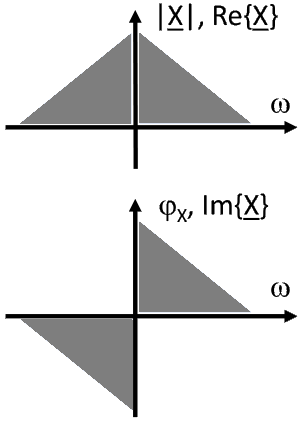
\includegraphics[width=0.3\columnwidth]{FT_Symmetrie.png}
	\end{wrapfigure}
		Realteil \& Betrag: \textbf{gerade}\\
		Imaginärteil \& Phase: \textbf{ungerade}.
	\[
	\underline{X}(-\omega) = \underline{X}^*(\omega)
	\]

		$x(t)$ reell \& gerade $\leftrightarrow$\\ $\underline{X}(\omega)$  reell \& gerade
		$$\underline{X}(\omega) = 2\int_0^\infty x(t)\cos(\omega t)\,dt$$
		$x(t)$ reell \& ungerade $\leftrightarrow$ $\underline{X}(\omega)$ imaginär \& ungerade
		$$\underline{X}(\omega) = -2j\int_0^\infty x(t)\sin(\omega t)\,dt$$
\end{mdframed}
